
Our evaluation consists of four parts, EcoDrive road testing results in both urban and highway environments, 
vehicle dynamics modeling accuracy, 
driving data statistics and trace-driven simulation. 


\subsection{Fuel Efficiency Test Results}


%\subsubsection{Test Drive Example}

\subsubsection{Urban}

\begin{figure}[!htbp]
\begin{center}
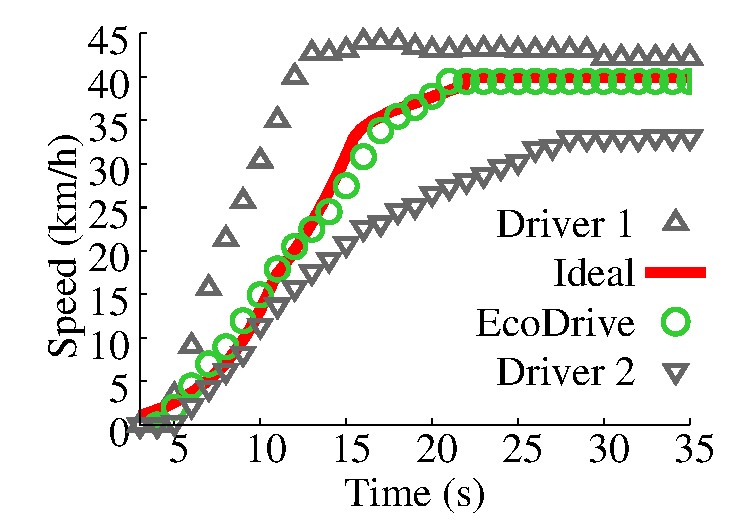
\includegraphics[width=3.0in,angle=0]{Figs/EcoDrive/evaluation/sampledrive240.pdf}
\vspace{-0.0cm}
\caption{Driving behaviors of EcoDrive and Human Drivers on a 300m length road segment.}
\vspace{-0.6cm}
\label{sampledrive}
\end{center}
\end{figure}


In this experiment, we compare EcoDrive with human drivers in urban
road segments.  
EcoDrive uses drive-by-wire technology to control air/fuel injection rate. 
It accelerates the vehicle by sending gas pedal position values to ECU. 
EcoDrive provides driver a switch button which can disable EcoDrive immediately. 
In our evaluation, we did not experience any bugs or out of control situations, 
but we made our risk management as follows. 
First, we control the input parameters. i.e., the gas pedal position value, 
on both the controller and the Arduino board. 
Second, we can shift the transmission to neutral or park to disconnect the engine and wheel
if the engine is out of control due to unexpected gas pedal position input. 
Third, the brake dominates the gas pedal and we can brake
even when the engine is out of control. 



\textbf{Test Drive Example}. 
A EcoDrive prototype test drive and human drive tests are conducted in a $300m$ length
road segment with speed limit of 25mph (or 40km/h). 
The vehicular speed traces are shown in Fig. \ref{sampledrive}. 
The ideal curve is plotted from the traces obtained from dynamic programming model. 
In our prototype, the air/fuel injection rate is controlled based
on sensed speed. 
The speed may change at any point during the query interval, 
so that it is challenge to control the air/fuel injection rate precisely at each speed. 
The differences between estimated speed traces and
actual speed traces are mainly caused by the impreciseness of 
speed sensing and road conditions.  
Some other factors affect the preciseness of vehicular speed 
control include wind speed and passenger
weights etc. 
Two human drivers are asked to drive 
on the same road segment. 
It is shown that the driver 1 is more aggressive by fast accelerations
and driver 2 is more conservative by slow accelerations. 
The driving trace of EcoDrive prototype falls in between. 
In this comparison, the prototype shows 23\% and 19\% fuel
efficiency improvements than driver 1 and 2, respectively. 
Driver can reach a fuel efficient speed faster by fast acceleration, 
but it takes more fuel during the acceleration process.  
If a driver uses lower accelerations to reduce fuel consumption
during acceleration process, overall fuel efficiency will not be increased due to driving in low (less fuel efficient) speeds
and longer travel time.
EcoDrive chooses the best strategy for economic driving. 


%\subsubsection{Urban Road Segments}


\begin{figure}[t]
\begin{center}
\vspace{-0.5cm}
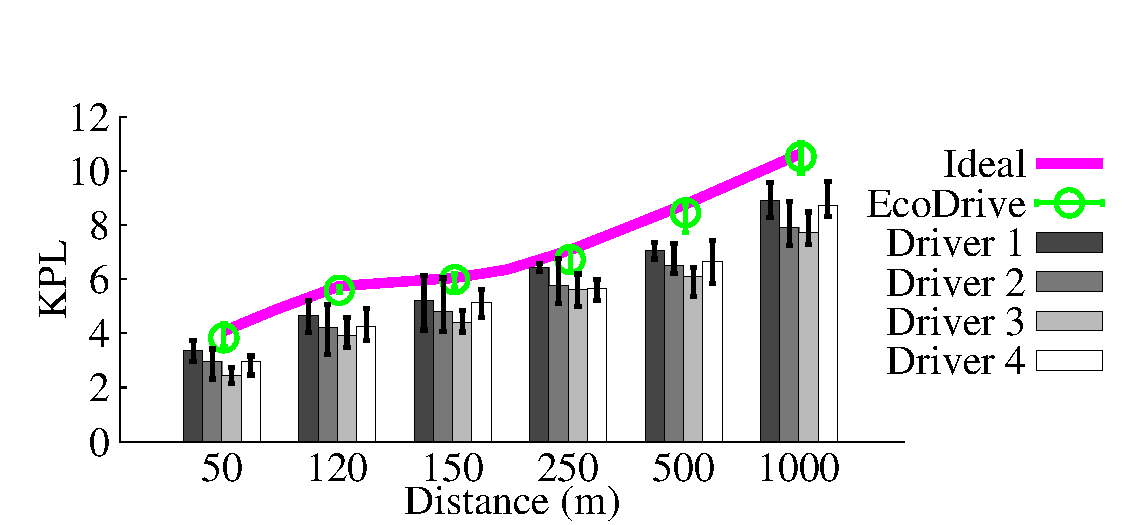
\includegraphics[width=3.0in,angle=0]{Figs/EcoDrive/evaluation/urbansegments.pdf}
\vspace{-0.0cm}
\caption{Fuel efficiency comparison between EcoDrive and human drivers on urban road segments. }
\vspace{-0.7cm}
\label{urbansegments}
\end{center}
\end{figure}

\textbf{Urban Road Segments}. 
We select six different road segments and let EcoDrive drive the car 10 times on each road segment. 
We recruited four drivers to drive on the same
road segments 10 times as well. 
The speed limit of the $500m$ and $1000m$ road segments
is $30mph$ (or $50km/h$) and the that of the $150m$
and $250m$ road segments is $25mph$ (or $40km/h$). 
There is no speed limit for the $50m$ and $120m$ road segments.
The length is the driving length of EcoDrive and 
the overall road segment length is longer so
that drivers have enough time to stop the car. 
The results are shown in Fig. \ref{urbansegments}. 
The ideal fuel consumption is the theoretical 
fuel consumption that is calculated based on AFR profile and dynamic programming model. 
The actual fuel consumption of EcoDrive on certain
road segment length is very stable. 
EcoDrive shows 10\%-40\% fuel efficiency improvement 
compared to different drivers with different road segment lengths. 
The fuel efficiency improvement comes from the smooth driving behaviors of EcoDrive. 
EcoDrive has an average of 20\% more travel time than human drivers.  
EcoDrive can have 5\%-10\% improvements than human drivers if not sacrificing travel time.
The plots of tradeoff between fuel consumption and travel time
are omitted due to the space limit. 

\subsubsection{Highway}


In this experiment, we compare EcoDrive with cruise control and human drivers
on highway. 

\begin{figure}[!htbp]
\begin{center}
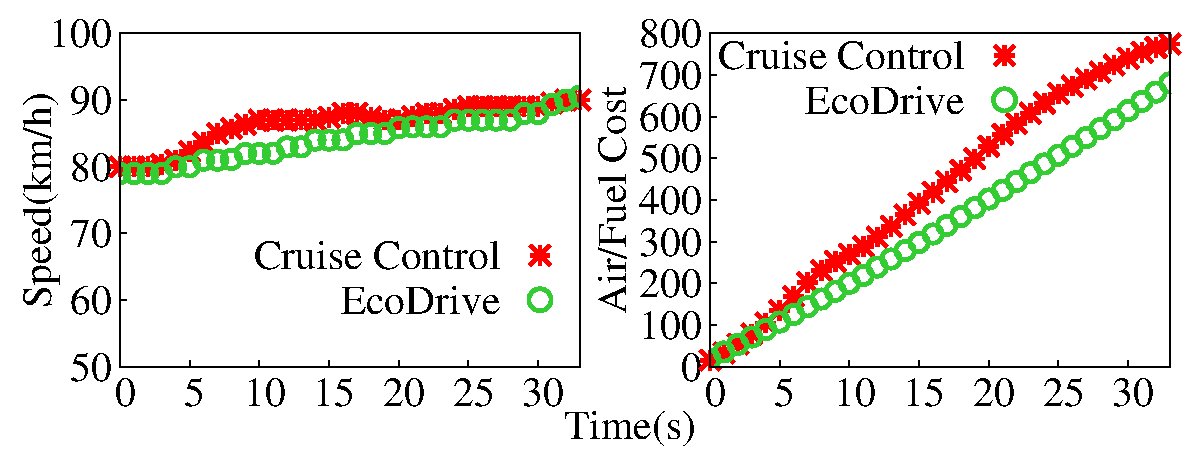
\includegraphics[width=5.0in,angle=0]{Figs/EcoDrive/evaluation/cruise_ecodrive_compare.pdf}
\vspace{-0.0cm}
\caption{Acceleration comparison between Cruise Control and EcoDrive. }
\vspace{-0.4cm}
\label{cruiseecodrive}
\end{center}
\end{figure}


\textbf{Compare to Cruise Control}. 
Fig. \ref{cruiseecodrive} plots the different acceleration patterns between cruise control
and EcoDrive. 
Cruise control is a vehicle built-in feature that can keep car driving
at a certain speed while human drivers can manually increase or decrease the cruising speed. 
The cruise control pattern is extracted when the gas pedal position is 0 but 
the air/fuel injection rate is higher than the idle state rate.  
As shown in the figure, cruise control consumes more
fuels than EcoDrive due to the aggressive acceleration strategy. 
The travel distance is similar for both cases, so EcoDrive is more fuel
efficient than cruise control. 
Similarly, driving uphill by using cruise control will consume more fuels as well. 
When the car is driving uphill, the vehicular speed drops due to grade resistance,
so cruise control will aggressively accelerate to the setting speed. 
In downhill conditions, cruise control will reduce air/fuel injection rate, 
while accelerating by maintaining the same air/fuel injection
rate has higher fuel efficiency. 


\begin{figure}[!htbp]
\begin{center}
\vspace{-0.4cm}
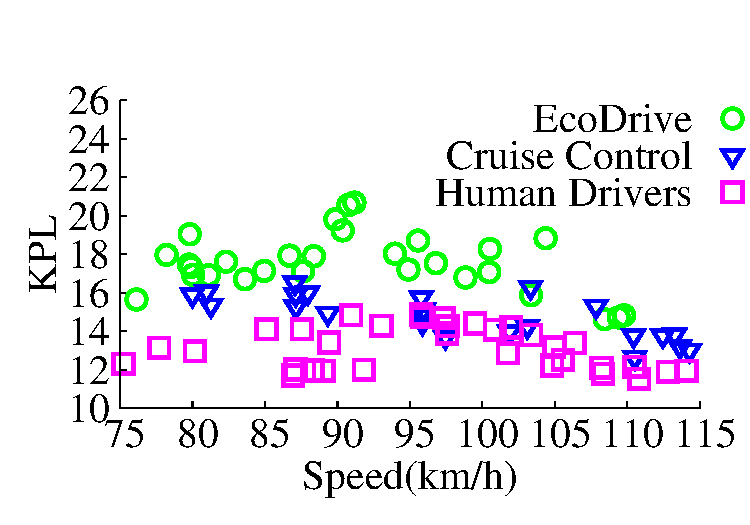
\includegraphics[width=3.0in,angle=0]{Figs/EcoDrive/evaluation/highway_ecodrive.pdf}
\vspace{-0.0cm}
\caption{Highway experiments.}
\vspace{-0.6cm}
\label{ecodrive_highway}
\end{center}
\end{figure}


\textbf{Compare to Human Drivers}. 
We evaluate EcoDrive by driving on two highway segments, 
one is a local highway segment and another is a cross state highway segment.  
The highway segments are selected based on historical driving traces of car 1. 
EcoDrive is evaluated by two-way driving in each highway segment, 
e.g., if EcoDrive enters highway at A and exits at B in one experiment
and it will enter at B and exits at A in next experiment.  
The two-way road testing is used to evaluate EcoDrive in both uphill
and downhill conditions. 
EcoDrive is evaluated between exit 256 and 262 on Madison's West Betline Highway, 
and between exit 132 and 136 on US 14 Highway.

The cruise control and human driving traces are extracted from 
historical driving traces collected on the same highway segments. 
In each driving trace, the car is traveling at a
constant speed(it may have some small speed variations). And we calculate the average speed of each trace as the vehicle speed.
The results are shown in Fig. \ref{ecodrive_highway}, where
each point represents the KPL of a $2km-3km$ length road segment. 
To eliminate the impact of traffic, the traces that 
have speed decrease due to brake are not included. 
In this experiment, EcoDrive shows more than 10\% fuel efficiency than cruise control
and more than 30\% fuel efficiency than human drivers on average. 



\subsubsection{Travel Time and Fuel Efficiency}

\nop{
\begin{figure}[!htbp]
\begin{center}
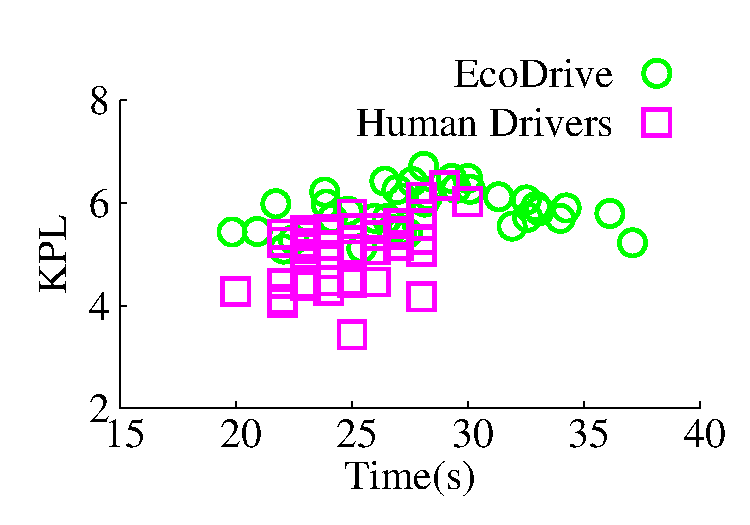
\includegraphics[width=1.7in,angle=0]{Figs/EcoDrive/evaluation/urban_timekpl.pdf}
\hspace{-0.5cm}
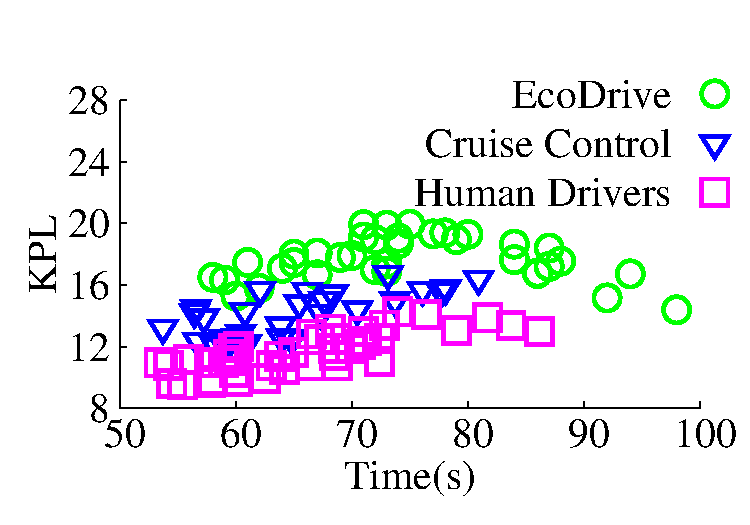
\includegraphics[width=1.7in,angle=0]{Figs/EcoDrive/evaluation/highway_timekpl.pdf}
\vspace{-0.2cm}
\caption{Trade off between travel time and fuel consumption in urban(left) and highway(right) environments.}
\vspace{-0.6cm}
\label{traveltime}
\end{center}
\end{figure}
}

\begin{figure}[!htbp]
\begin{center}
\vspace{-0.4cm}
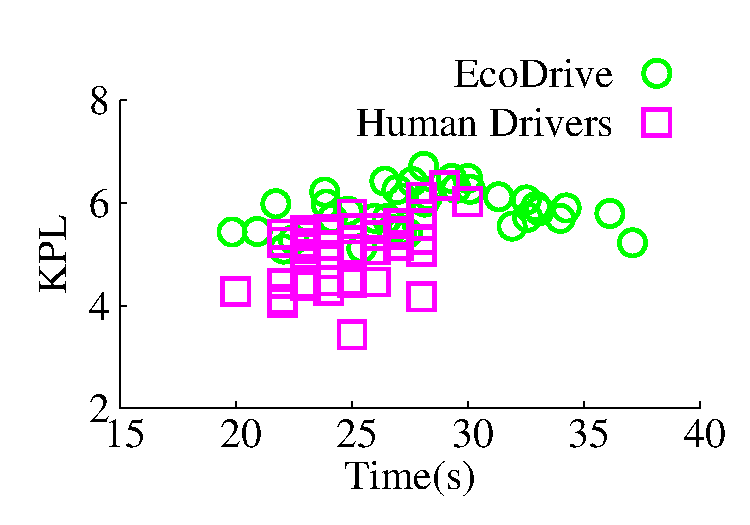
\includegraphics[width=3.0in,angle=0]{Figs/EcoDrive/evaluation/urban_timekpl.pdf}
\vspace{-0.0cm}
\caption{Tradeoff between travel time and fuel consumption on a 250m road segment.}
\vspace{-0.6cm}
\label{tradeoff_urban}
\end{center}
\end{figure}

\begin{figure}[!htbp]
\begin{center}
\vspace{-0.4cm}
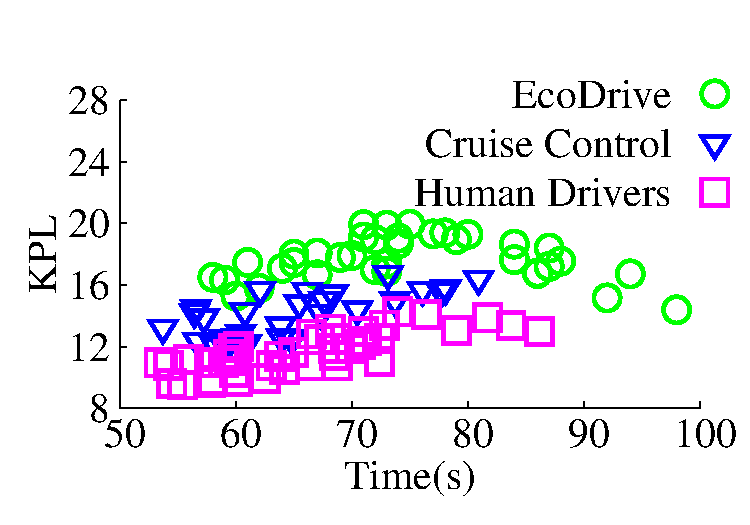
\includegraphics[width=3.0in,angle=0]{Figs/EcoDrive/evaluation/highway_timekpl.pdf}
\vspace{-0.0cm}
\caption{Tradeoff between travel time and fuel consumption on highway.}
\vspace{-0.6cm}
\label{tradeoff_highway}
\end{center}
\end{figure}

In this experiment, we evaluate the tradeoff between travel time and fuel consumption. 

\textbf{Urban}. 
The tradefoff between travel time and fuel consumption of EcoDrive on $250m$ 
road segment is shown in Fig. \ref{tradeoff_urban}. For EcoDrive, the optimal KPL is around 7 and the 
travel time is around 28 seconds. On the other hand, the average KPL for human 
drivers is around 5.5 and the average travel time is around 25 seconds. 
EcoDrive can achieve a 20\% fuel efficiency improvement 
on average by sacrificing travel time by around 10\%. 
EcoDrive can also improve fuel efficiency under same travel time in most cases. 

\textbf{Highway}.  
Fig. \ref{tradeoff_highway} shows the tradeoff between travel time and fuel efficiency on highway. 
Each highway segment length is around $2km-3km$. 
EcoDrive can improve fuel efficiency by more than 30\% on average without sacrificing travel time.    
The gain comes from smooth acceleration and road adaptation. 
More fuel efficiency can be achieved by cruising at the peak KPL speed, 
which is around $90km/h$ in this evaluation. 

\subsection{Modeling Accuracy}


\begin{figure}[!htbp]
\begin{center}
\vspace{-0.2cm}
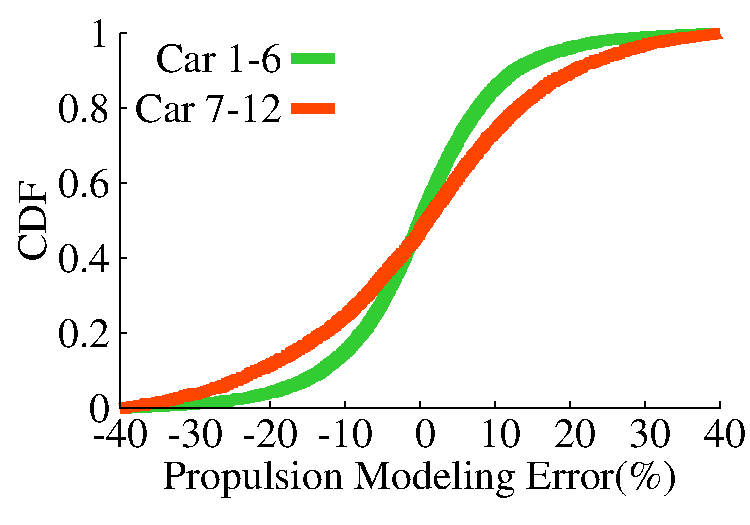
\includegraphics[width=2.2in,angle=0]{Figs/EcoDrive/evaluation/propulsion_error_cdf_2.pdf}
\vspace{-0.2cm}
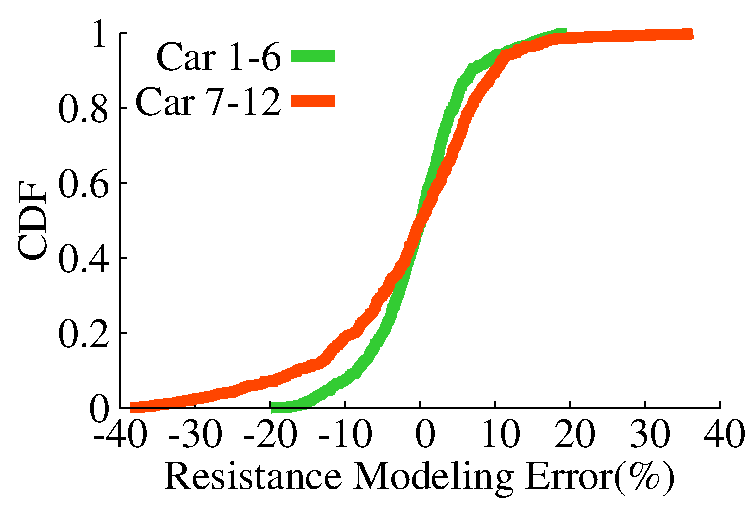
\includegraphics[width=2.2in,angle=0]{Figs/EcoDrive/evaluation/resistance_error_cdf_2.pdf}
\vspace{-0.2cm}
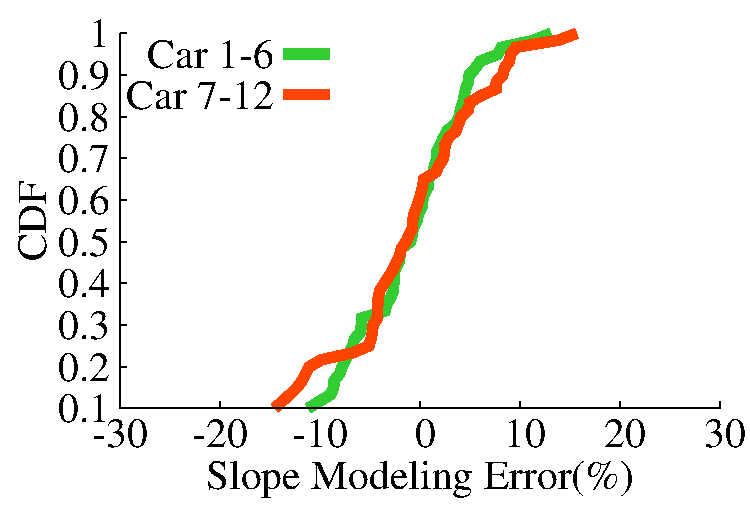
\includegraphics[width=2.2in,angle=0]{Figs/EcoDrive/evaluation/slope_error_cdf_2.pdf}
\vspace{-0.2cm}
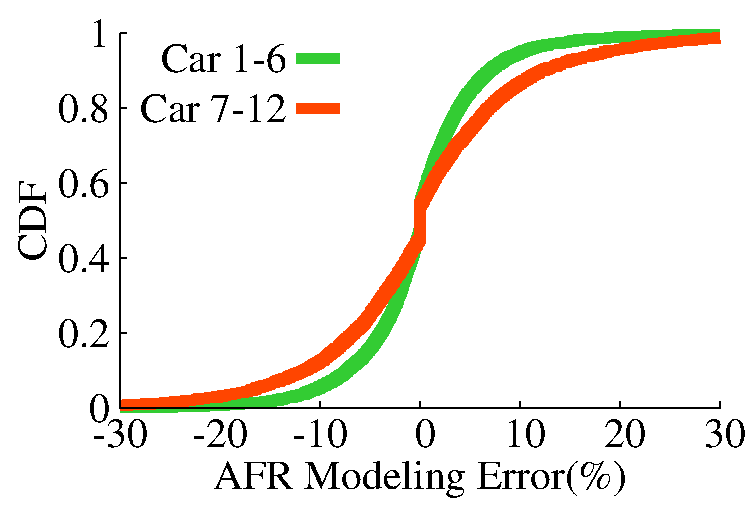
\includegraphics[width=2.2in,angle=0]{Figs/EcoDrive/evaluation/afr_profile_error_cdf_2.pdf}
\caption{The cumulative distribution function of vehicle dynamics modeling errors.}
\vspace{-0.6cm}
\label{modelingaccuracy}
\end{center}
\end{figure}

In this experiment, we evaluate the modeling accuracy of vehicle dynamics models. 
Different vehicle forces, propulsion, resistance and grade resistance, are
evaluated separately. 
The AFR profile calculation accuracy is evaluated as well. 
We divide the data into two sets, one set is the training set 
used to build the model and another set is the testing set
for evaluating the model. 
For each model, we repeat this process and plot the 
modeling accuracy of various vehicle dynamics models in Fig. \ref{modelingaccuracy}. 
From top-left to bottom-right, they are propulsion model evaluation, 
drivetrain loss and wind resistance model evaluation, 
grade resistance model evaluation, 
and AFR profile evaluation. 


We use \textcolor{green}{\textbf{green}} curves to represent the cars have more than one thousand miles
driving traces (Car 1-6) and use \textcolor{red}{\textbf{red}} curves to represent the rest (Car 7-12). 
The \textcolor{green}{\textbf{green}} curves show that the fitting errors of 
more than $95\%$ cases are within $\pm10\%$. 
The \textcolor{red}{\textbf{red}} curves show less fitting accuracy 
due to less miles. 




\subsection{Driving Data Statistics}

\subsubsection{Urban Road Segment Length}

\begin{figure}[!htbp]
\begin{center}
\vspace{-0.3cm}
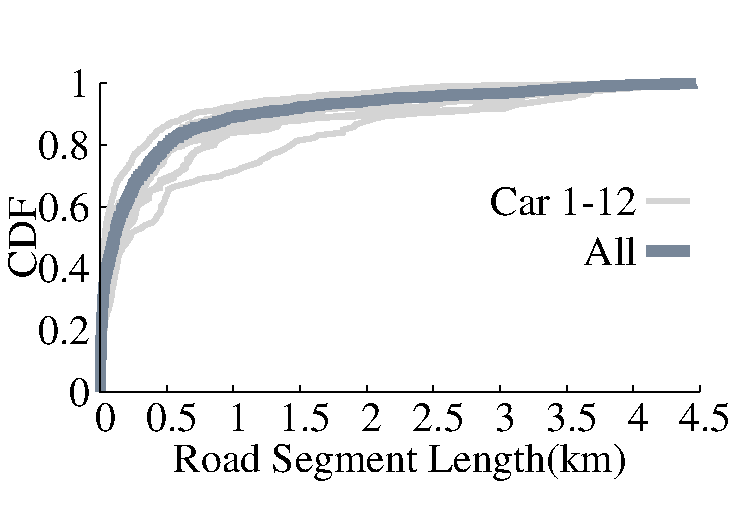
\includegraphics[width=3.0in,angle=0]{Figs/EcoDrive/evaluation/urban_road_segment.pdf}
\vspace{-0.0cm}
\caption{Road segment length in urban area.}
\vspace{-0.8cm}
\label{urbanroad}
\end{center}
\end{figure}

We summarize the length of road segments in Fig. \ref{urbanroad}.
A road segment is defined as the distance between two stand/stop locations. 
A stand/stop location is defined as following: 
1) The speed of the car is zero; 2) The car is making a turn. 
The speed of the car can be easily sensed from the OBD port. 
We identify turns from GPS data. 
The driving direction of car can be calculated from two adjacent GPS points. 
If the accumulated driving direction change are close to $90$ degree, 
then we mark this is a stand/stop location. 
This rough road segment length statistics give us a 
guideline for experiments. 
As shown in the figure, the most of road segments are within 1000m.
This indicates that the driving pattern in urban area is primarily  
accelerate-brake. 


\subsubsection{Urban Acceleration}



\begin{figure}[!htbp]
\begin{center}
%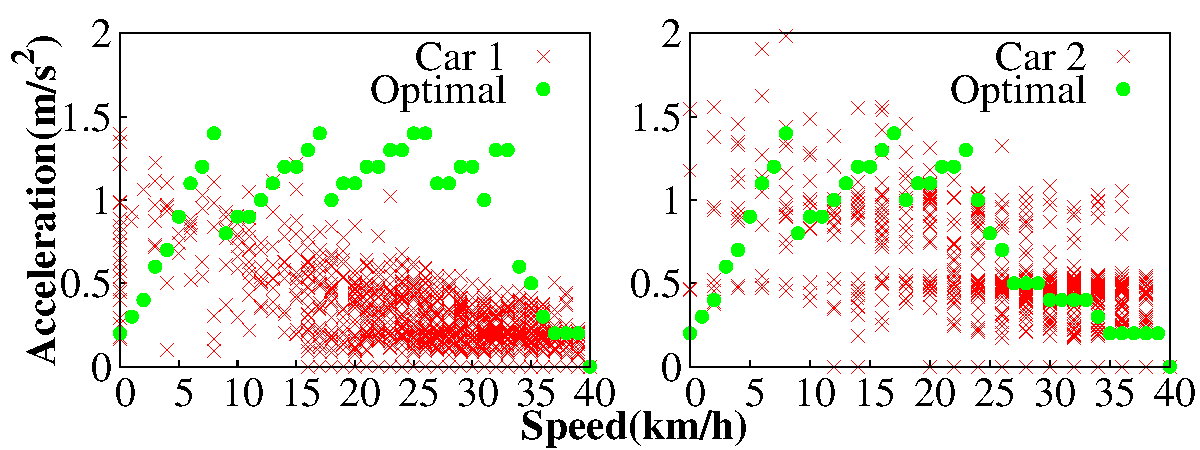
\includegraphics[width=3.2in,angle=0]{Figs/EcoDrive/evaluation/urban_accelerations.pdf}
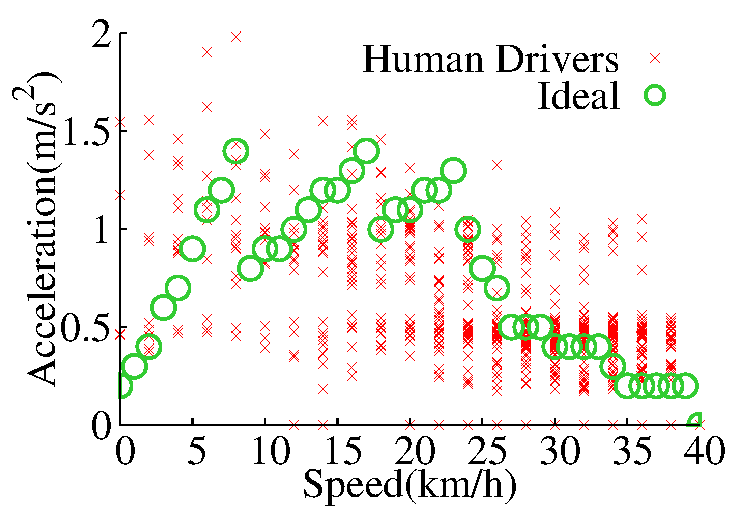
\includegraphics[width=3.0in,angle=0]{Figs/EcoDrive/evaluation/real_opt_acce_single.pdf}
\vspace{-0.0cm}
\caption{The urban acceleration patterns of different drivers.}
\vspace{-0.5cm}
\label{urbanaccelerations}
\end{center}
\end{figure}

Fig. \ref{urbanaccelerations} explains the acceleration patterns of
car 1 and the ideal acceleration pattern calculated by EcoDrive
with equal road length. 
As shown in the figure, drivers are not aware of the most efficient
accelerations of different speeds and not able to drive at a certain speed. 
They drive either lower than
desired accelerations, which will increase fuel consumption
due to longer travel time in low KPL speeds, 
or higher than desired accelerations, 
which will increase fuel consumption due to extra fuel consumption
to achieve the target speed. 



\subsubsection{Highway Driving Speed}






\begin{figure}[!htbp]
\begin{center}
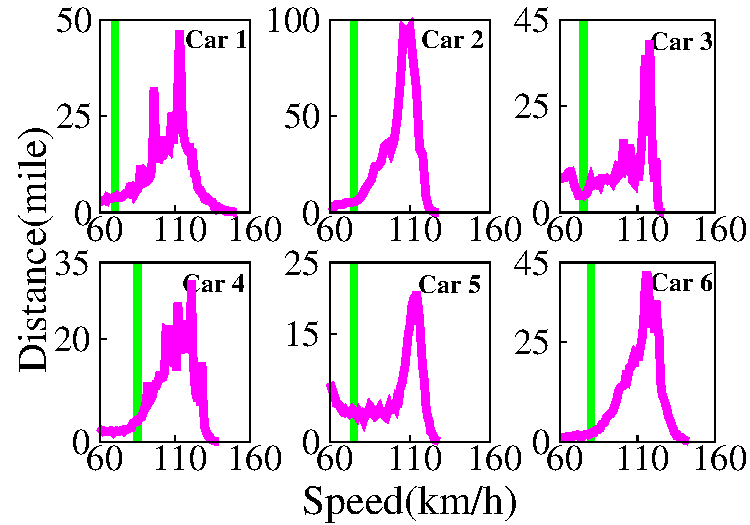
\includegraphics[width=3.0in,angle=0]{Figs/EcoDrive/evaluation/hwy_speeds.pdf}
\vspace{-0.0cm}
\caption{The highway driving speed distributions of car 1-6.}
\vspace{-0.6cm}
\label{highwayspeeds}
\end{center}
\end{figure}

The speed limits of rural highway is $65mph$ ($104.6km/h$) 
to $70mph$ ($112.6km/h$), and
the speed limit of urban highway is $55mph$ ($88.5km/h$). 
We summarize the highway driving speeds of car 1-6 
and illustrate the distribution and best KPL speed in Fig. \ref{highwayspeeds}. 
We observe that most drivers drive above the speed limits with
noticeable mileages and much higher than the best KPL speed. 
This is partially because the drivers are not aware of
the much higher fuel consumption in high speeds. 
Also, slowing down when following a slow car 
will increase fuel consumption due to power loss when braking. 
Frequent accelerations and decelerations increase
fuel consumption as well. 

\subsection{Trace-driven Simulation}


\begin{figure}[!htbp]
\begin{center}
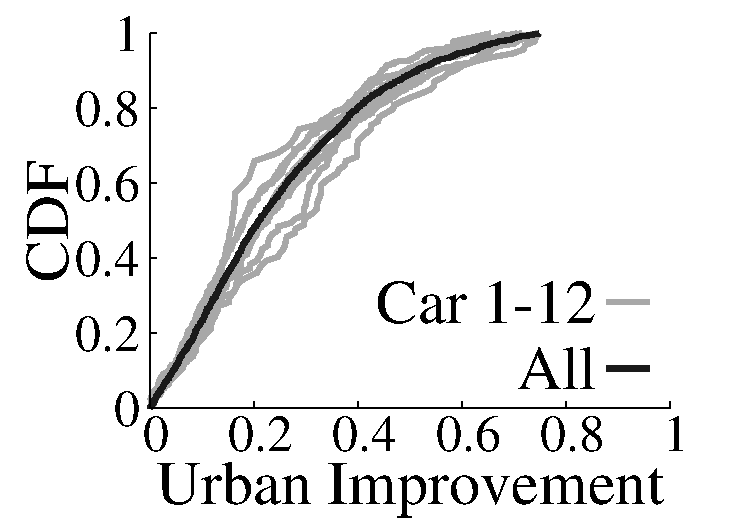
\includegraphics[width=2.0in,angle=0]{Figs/EcoDrive/evaluation/urban_cdf_all.pdf}
\hspace{-0.5cm}
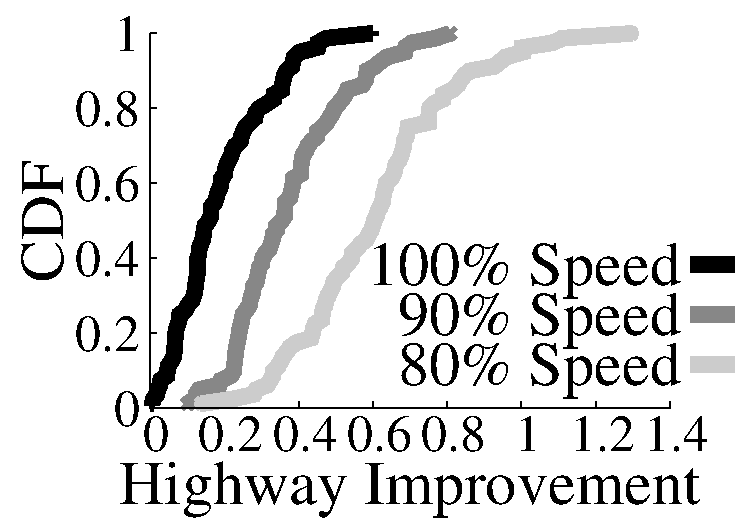
\includegraphics[width=2.0in,angle=0]{Figs/EcoDrive/evaluation/hwy_improve_cdf.pdf}
\vspace{-0.2cm}
\caption{Fuel efficiency improvements by trace-driven simulation.}
\vspace{-0.6cm}
\label{tracedriven}
\end{center}
\end{figure}

In this experiment, we evaluate EcoDrive by trace-driven simulations. 

\textbf{Urban}. We divide urban trips into variable-length road segments 
where the vehicular speed is 0 at the start and end of each segment. 
Each segment is divided into four parts, accelerating part, cruising part, 
braking part and idle part. 
Accelerating part ended when the speed does not increase in 5 seconds. 
Braking part started when the driver release gas pedal at the end of each segment. 
Cruising part falls between accelerating part and braking part.
Idle part follows braking part after the vehicular speed reach 0.  
The speed limit is calculated based on the average speed of cruising part. 
We calculate the fuel cost of EcoDrive by replaying acceleration and cruising parts.
We use the same braking and idle cost extracted from original traces.
We sum up the two costs to calculate the final fuel consumption of EcoDrive. 
As shown in Fig. \ref{tracedriven}, EcoDrive can improve a median of 
20\% fuel efficiency in urban environment. 
The travel time is reduced by 10\%-30\% in 20\% cases and is increased
by less than 25\% in 60\% cases. 
The plots of travel time are omitted due to the space limit.   

\textbf{Highway}.  
We divide highway trips into road segments based on deceleration.
If the deceleration is larger than a threshold, we separate current
segment into one highway segment.
The average speed of highway segment is used as target speed for EcoDrive. 
We replay each highway segment by EcoDrive with three different
target speeds, the same target speed, 90\% of target speed and
80\% of target speed. 
As shown in Fig. \ref{tracedriven}, EcoDrive can improve
fuel efficiency by more than 20\% on average without sacrificing 
travel time and can improve an average of 40\% fuel efficiency
by sacrificing 10\% travel time on highway. 


   

 
